% ======================================================================
%  ClassRoomSTORM Theory Notes (V2 documentation)
%  Companion to ClassRoomSTORM Studio V1.2.
%  Self-contained LaTeX source. Compile from this directory with:
%      pdflatex ClassRoomSTORM_Theory.tex   (run twice)
%  The bibliography is embedded (no bibtex/biber needed).
%  Figures live in ../figures/theory/.
% ======================================================================
\documentclass[11pt,a4paper]{article}

\usepackage[utf8]{inputenc}
\usepackage[T1]{fontenc}
\usepackage{lmodern}
\usepackage{amsmath,amssymb}
\usepackage{geometry}
\usepackage{graphicx}
\usepackage[font=small,labelfont=bf]{caption}
\usepackage{booktabs}
\usepackage{tabularx}
\usepackage{enumitem}
\usepackage{xcolor}
\usepackage{tcolorbox}
\tcbuselibrary{breakable}
\usepackage{hyperref}
\usepackage{cleveref}

\geometry{margin=24mm}
% Keep figure-only pages aligned at the top with a deliberate inter-float gap.
\makeatletter
\setlength{\@fptop}{0pt}
\setlength{\@fpsep}{16pt plus 2pt minus 2pt}
\setlength{\@fpbot}{0pt plus 1fil}
\makeatother
\graphicspath{{../figures/theory/}{../figures/help/}{figures/theory/}{figures/help/}}
\hypersetup{colorlinks=true, linkcolor=blue!45!black, urlcolor=blue!45!black,
  citecolor=blue!45!black,
  pdftitle={ClassRoomSTORM Theory Notes},
  pdfauthor={Awanish Pratap Singh},
  pdfsubject={Physics of localization-based super-resolution microscopy}}
\setlist[itemize]{itemsep=2pt, topsep=4pt}
\setlist[enumerate]{itemsep=3pt, topsep=4pt}

\DeclareMathOperator{\erf}{erf}
\newcommand{\Var}{\operatorname{Var}}

% ---- Callout boxes --------------------------------------------------
\newtcolorbox{csnote}[1][Note]{breakable, colback=blue!4, colframe=blue!55!black,
  fonttitle=\bfseries, coltitle=white, title={#1}, boxrule=0.5pt, arc=2pt}
\newtcolorbox{cswarn}[1][Scope and limitations]{breakable, colback=red!5,
  colframe=red!60!black, fonttitle=\bfseries, coltitle=white, title={#1},
  boxrule=0.5pt, arc=2pt}
\newtcolorbox{csideal}[1][The statistical ideal (background only)]{breakable,
  colback=violet!5, colframe=violet!55!black, fonttitle=\bfseries,
  coltitle=white, title={#1}, boxrule=0.5pt, arc=2pt}
\newtcolorbox{csderiv}[1][Derivation (optional)]{breakable, colback=gray!8,
  colframe=gray!55!black, fonttitle=\bfseries, coltitle=white, title={#1},
  boxrule=0.5pt, arc=2pt}

\newcommand{\file}[1]{\texttt{#1}}
\newcommand{\app}{ClassRoomSTORM}

\title{\textbf{\app{} Theory Notes}\\[2pt]\large Diffraction, Blinking, and the
       Physics of Localization Microscopy}
\author{Awanish Pratap Singh}
\date{Companion to \app{} Studio, software version 1.2}

% ======================================================================
\begin{document}
\maketitle
\thispagestyle{empty}

\begin{abstract}
\noindent These notes explain the physics behind \app{} Studio V1.2. They proceed from the diffraction limit of an ordinary microscope to the idea of
localization microscopy: why a blurred spot can still be \emph{located} far more
precisely than it can be \emph{resolved}, and how many such locations accumulate
into a sharp image. The central distinction is between two quantities: \emph{resolution} (how finely an instrument separates two points in a single snapshot) is set by optical blur, whereas \emph{localization precision} (how well the centre of one isolated spot is known) is a
statistical quantity set by photon counts, background, and noise. The final
sections describe how \app{} V1.2 reconstructs an image, and explain the capabilities and limitations of the centroid method. The V1.2 release adds
calibrated coordinate export, crop-aware truth validation, fractional-coordinate
rendering, and optional frame-median subtraction while retaining the straightforward centroid reconstruction method.
\end{abstract}

\begingroup\small\tableofcontents\endgroup
\newpage

% ======================================================================
\section{Introduction: The Resolution Problem}
\label{sec:intro}

A microscope cannot show arbitrarily fine detail. Two points of light that are
close enough together blur into a single spot, even with an ideal lens.
This limit, the \emph{diffraction limit}, has been understood since the
nineteenth century~\cite{abbe1873} and is roughly half the wavelength of
light, about $200$-$250$~nm for visible light~\cite{bechhoefer2015,
schermelleh2019}.

For more than a century this was considered an unbreakable barrier. Modern
\emph{super-resolution} microscopy sidesteps it. One family of methods, \emph{single-molecule localization microscopy} (SMLM), which includes STORM and PALM, uses a simple statistical principle: never let two nearby
emitters be visible at the same time. If only a few, well-separated emitters
glow in any one frame, each appears as an isolated blurred spot, and the
\emph{centre} of an isolated spot can be estimated very precisely. Repeating this
over thousands of frames and accumulating the centres yields a far sharper
picture than any single frame~\cite{huang2010, sigal2018}.

\app{} is a teaching application that reproduces the \emph{statistical and
computational logic} of SMLM. Its \emph{Virtual Experiment} generates blinking
videos with controllable blur, brightness, and noise; its \emph{SR
Reconstruction} workflow locates the spots and accumulates them. These notes
explain the physics underlying the software. They are meant to be read alongside
the \emph{\app{} Help} document, which explains the buttons and screens.

\begin{csnote}[A note on scope]
\app{} is a learning tool. It is not a fluorescence microscope, and its
reconstruction uses a deliberately simple estimator rather than a
research-grade one. Throughout these notes, material describing the
\emph{ideal} statistical method is clearly marked in violet boxes; the running
text and \cref{sec:pipeline} describe what \app{} V1.2 actually does.
\end{csnote}

% ======================================================================
\section{The Diffraction Limit}
\label{sec:diffraction}

When light from a single point passes through a lens of finite size, diffraction
spreads it into a small pattern of rings called the \emph{Airy pattern}:
\begin{equation}
  I(r) = I_0\left[\frac{2J_1(\alpha r)}{\alpha r}\right]^{2},
  \qquad \alpha = \frac{2\pi\,\mathrm{NA}}{\lambda},
  \label{eq:airy}
\end{equation}
where $r$ is the radial distance from the centre, $I_0$ is the peak intensity,
$J_1$ is the first-order Bessel function, $\lambda$ is the wavelength of light,
and $\mathrm{NA}$ is the \emph{numerical aperture} of the lens (a measure of how
wide a cone of light it collects). A perfect point of light is therefore never
imaged as a point; it appears as a small bright disc.

Two points can be distinguished only if their discs do not overlap too much. Abbe's
criterion gives the smallest resolvable separation~\cite{abbe1873,
bechhoefer2015}:
\begin{equation}
  d_{\mathrm{Abbe}} \simeq \frac{\lambda}{2\,\mathrm{NA}}.
  \label{eq:abbe}
\end{equation}
A closely related statement, the Rayleigh criterion, places the threshold where
the peak of one Airy disc falls on the first dark ring of the
other~\cite{bechhoefer2015, prakash2024}:
\begin{equation}
  d_{\mathrm{Rayleigh}} \simeq \frac{0.61\,\lambda}{\mathrm{NA}}.
  \label{eq:rayleigh}
\end{equation}

\begin{csnote}[Worked example]
Consider green light with $\lambda \approx 550$~nm, and an objective with
$\mathrm{NA}\approx 1.4$. Then $d_{\mathrm{Abbe}} \approx 550/(2\times1.4)
\approx 196$~nm and $d_{\mathrm{Rayleigh}} \approx 0.61\times550/1.4 \approx
240$~nm. This is the few-hundred-nanometre barrier that super-resolution methods
must overcome.
\end{csnote}

\Cref{fig:rayleigh} shows how two emitters merge as their separation shrinks
toward this limit. The key point is that
\cref{eq:abbe,eq:rayleigh} describe \emph{resolution}, the ability to
separate two points that are visible \emph{at the same time}. They say nothing
about how well the position of a \emph{single, isolated} point can be measured.
A single point can be located much more precisely than two points can be resolved.

\begin{figure}[htbp]
  \centering
  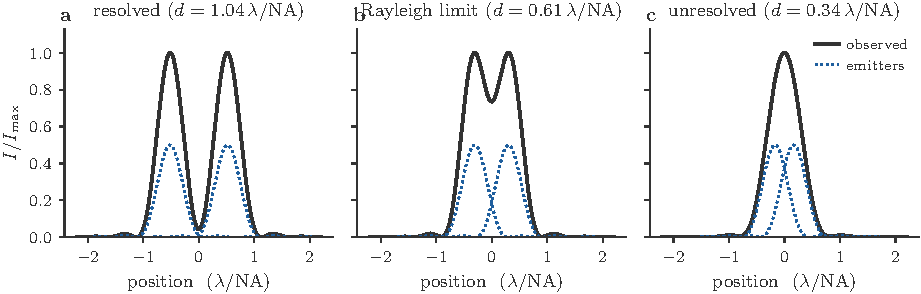
\includegraphics[width=\linewidth]{T2_rayleigh}
  \caption{Two incoherent point sources of equal brightness imaged through an ideal circular pupil. Each panel uses the same normalization for the sum and both component PSFs, so the components add to the plotted sum. Rayleigh separation is $0.610\,\lambda/\mathrm{NA}$; it is a conventional two-point criterion, not a universal localization limit.}
  \label{fig:rayleigh}
\end{figure}

% ======================================================================
\section{The Point Spread Function}
\label{sec:psf}

The image of a single point source is called the \emph{point spread function}
(PSF). The Airy pattern of \cref{eq:airy} is the exact PSF of an ideal lens, but
for calculations a simpler model is almost always used: a two-dimensional
Gaussian~\cite{thompson2002, small2014}. An isolated emitter is modelled as
\begin{equation}
  I(x,y) = b + \frac{N}{2\pi\sigma^{2}}
           \exp\!\left[-\frac{(x-x_0)^2 + (y-y_0)^2}{2\sigma^{2}}\right],
  \label{eq:gauss}
\end{equation}
where $(x_0,y_0)$ is the true emitter position, $N$ is the total number of
signal photons, $b$ is a background level, and $\sigma$ is the \emph{width} of
the PSF. The width is set by the optics and the pixel size $a$ of the camera; a
useful approximate relation is~\cite{thompson2002}
\begin{equation}
  \sigma \approx 0.21\,\frac{\lambda}{\mathrm{NA}\cdot a}.
  \label{eq:sigma}
\end{equation}
The Gaussian is not exact because it ignores the Airy rings, but it captures the
central peak well (\cref{fig:airy}) and makes the algebra of localization
tractable.

In \app{}, the \emph{Virtual Experiment} renders each blinker as a Gaussian
spot, and you set its width directly with the \texttt{sigma\_px} control.
Choosing a large $\sigma$ is the same as building a more strongly
diffraction-limited ``microscope.''

\begin{figure}[htbp]
  \centering
  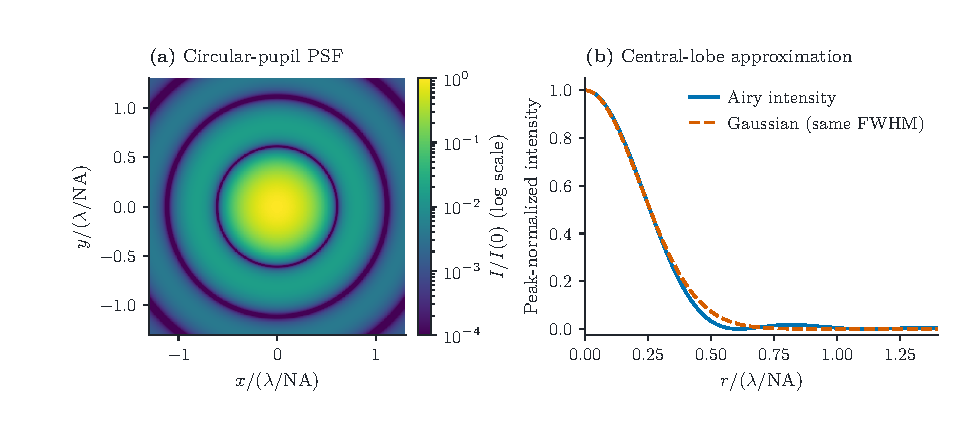
\includegraphics[width=\linewidth]{T1_airy_gaussian}
  \caption{Ideal scalar, incoherent circular-pupil PSF. The image uses a labelled logarithmic colour scale to reveal rings; the profile is linear. The Gaussian matches the Airy FWHM only, not the side lobes or total energy.}
  \label{fig:airy}
\end{figure}

% ======================================================================
\section{Image Formation and Sampling}
\label{sec:formation}

A real image is the true scene blurred by the PSF and then corrupted by noise.
Writing the true distribution of light as $f(x,y)$, the PSF as $h(x,y)$, and the
noise as $\eta(x,y)$, the recorded image is
\begin{equation}
  g(x,y) = (h * f)(x,y) + \eta(x,y),
  \label{eq:convolution}
\end{equation}
where $*$ denotes convolution. Convolution by $h$ describes the blurring discussed in
\cref{sec:diffraction}: every point in $f$ is replaced by a copy of the PSF, as
\cref{fig:formation} illustrates.

A camera does not sample $g$ at infinitely fine points. Each pixel
\emph{collects all the light that lands on its small square}. The expected number
of counts in the pixel at column $j$, row $i$, for a single Gaussian emitter,
is the Gaussian \emph{integrated} over that pixel~\cite{mortensen2010}:
\begin{equation}
  M_{ij} = b + N\,G_x(j;x_0,\sigma)\,G_y(i;y_0,\sigma),
  \label{eq:pixmodel}
\end{equation}
\begin{equation}
  G_x(j;x_0,\sigma) = \tfrac{1}{2}\left[
    \erf\!\frac{j+\tfrac12-x_0}{\sqrt{2}\,\sigma}
    - \erf\!\frac{j-\tfrac12-x_0}{\sqrt{2}\,\sigma}\right],
  \label{eq:erf}
\end{equation}
with $G_y$ defined the same way along the rows. The factor $G_x$ is simply the
fraction of the Gaussian's light that falls within the width of pixel $j$;
$\erf$ is the error function. \Cref{eq:pixmodel,eq:erf} give the
\emph{forward model}: they say what the camera \emph{should} record, on average,
for an emitter at $(x_0,y_0)$. Localization, in \cref{sec:locating}, is the inverse problem of estimating the emitter position from the recorded image.

\begin{figure}[htbp]
  \centering
  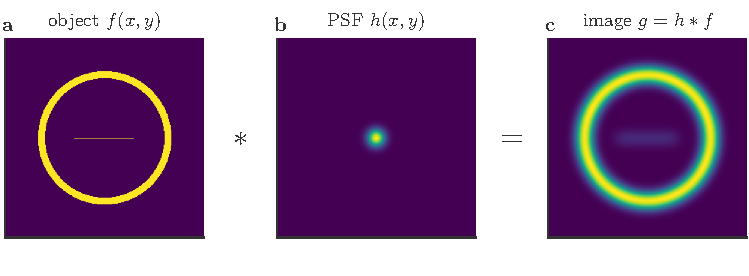
\includegraphics[width=\linewidth]{T3_image_formation}
  \caption{Linear shift-invariant, incoherent image formation: two equal point sources convolved with a normalized Gaussian PSF. Pixel integration is a subsequent detector operation. The brightness in each panel is scaled independently; the circles identify source positions.}
  \label{fig:formation}
\end{figure}

% ======================================================================
\section{Photon Noise}
\label{sec:noise}

Light arrives as discrete photons at random times. If the expected count in a pixel is $M_{ij}$, the number it \emph{actually} records, $Z_{ij}$, fluctuates
according to Poisson statistics~\cite{ober2004}:
\begin{equation}
  Z_{ij} \sim \mathrm{Poisson}(M_{ij}).
  \label{eq:poisson}
\end{equation}
A defining property of the Poisson distribution is that its variance equals its
mean. Real cameras add a second source of noise, electronic noise (\emph{read noise}) to the photon noise, so
the total per-pixel variance is approximately~\cite{lelek2021}
\begin{equation}
  \Var[Z_{ij}] \approx M_{ij} + \left(\frac{\sigma_{\mathrm{read}}}{g}\right)^{2},
  \label{eq:variance}
\end{equation}
where $\sigma_{\mathrm{read}}$ is the camera read noise and $g$ its gain.

Photon noise imposes a fundamental \emph{precision limit} (\cref{sec:precision}). The more
photons an emitter delivers, the smaller the relative fluctuations, and the more
precisely its position can be estimated. \Cref{fig:noise} shows how repeated
measurements of the same emitter scatter because of this noise. In \app{}, the
\texttt{Brightness} control sets the photon budget $N$ and \texttt{Read noise}
sets $\sigma_{\mathrm{read}}$, so students can observe how precision improves as they increase brightness.

\begin{figure}[htbp]
  \centering
  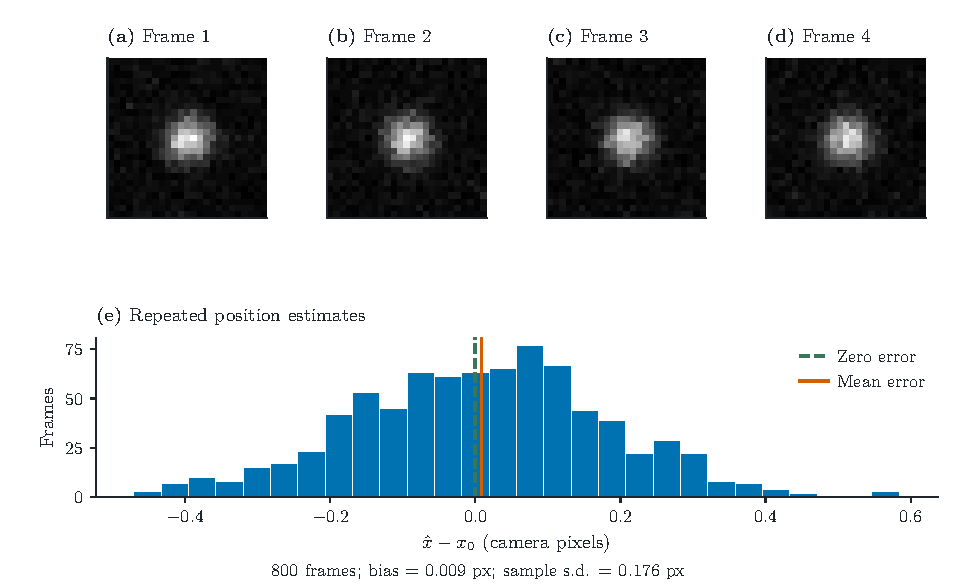
\includegraphics[width=\linewidth]{T5_poisson_noise}
  \caption{Pixel-integrated Gaussian signal with 2000 expected photons, $\sigma=2.3$ pixels, and a Poisson background with a mean of 3 counts/pixel. The V1.2 single-emitter centroid uses $q=0.98$ and frame-median subtraction. The histogram shows the spread and bias of repeated estimates, not per-event uncertainty.}
  \label{fig:noise}
\end{figure}

% ======================================================================
\section{Blinking and Single-Molecule Localization Logic}
\label{sec:blinking}

The central idea is to separate nearby emitters in time. Suppose a sample contains many emitters packed more
closely than the diffraction limit. If they all glow at once, their PSFs overlap
and \cref{eq:convolution} produces an unresolvable blur because of the diffraction limit (\cref{fig:blinking}a).

But suppose instead that the emitters \emph{blink}: at any instant only a small,
random subset is switched on, and those that are on happen to be far apart. Then
each frame contains only a few \emph{isolated} spots (\cref{fig:blinking}b).
Each isolated spot can be located precisely (\cref{sec:locating}). Over thousands
of frames, different emitters become active, and the accumulated set of
locations traces out the whole structure.

This is single-molecule localization microscopy. STORM~\cite{rust2006} and
PALM~\cite{betzig2006}, both introduced in 2006, use photoswitchable dyes and
fluorescent proteins to make molecules blink; the same logic underlies the
broader field of far-field optical nanoscopy~\cite{hell2007, lelek2021}. The diffraction limit is never actually \emph{broken}: it is
\emph{sidestepped}, by arranging that two unresolved emitters are never on at the
same time. (Other super-resolution methods, such as STED~\cite{hell1994}, take a
different route by physically sharpening the PSF.)

\app{} reproduces this logic. The \emph{Virtual Experiment} builds exactly such
blinking videos: you choose how many emitters may be on per frame and how far
apart they must be. The companion macroscopic experiment uses blinking LEDs in
place of fluorophores: emitters that are large in physical size but produce
data with the \emph{same statistical structure} as SMLM. Low-cost real SMLM
instruments built in the same spirit have been described in the
literature~\cite{danial2022, ma2017}.

\begin{figure}[htbp]
  \centering
  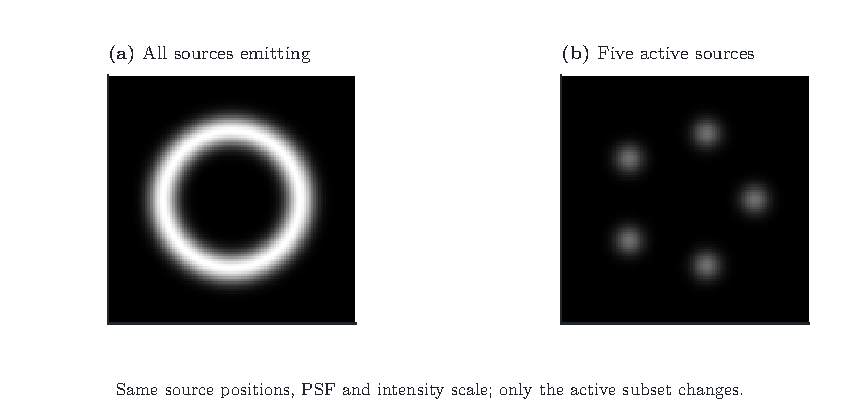
\includegraphics[width=0.90\linewidth]{T4_blinking}
  \caption{Temporal sparsity: the same emitter arrangement with all 40 sources active or five well-separated sources active. These are noise-free expectations with one shared intensity scale; sparse activation enables individual localization.}
  \label{fig:blinking}
\end{figure}

\begin{csnote}[Why separation matters]
Localization works \emph{only} when spots are isolated. If two emitters are on
together and their PSFs overlap, the methods in \cref{sec:locating} return one
position somewhere between them, giving one incorrect position rather than two correct positions. This is
why the \emph{Virtual Experiment} lets you control \texttt{Max blinkers/frame}
and \texttt{Blinker spacing}, and why crowded data reconstruct poorly.
\end{csnote}

% ======================================================================
\section{Localizing an Emitter}
\label{sec:locating}

Given one isolated, blurred spot, where is its centre? This section gives the simple method \app{} V1.2 uses, the precision that method can achieve, and, as clearly marked background, the statistically optimal approach.

% --------------------------------------------------------------------
\subsection{The centroid estimator used in V1.2}
\label{sec:centroid}

\app{} V1.2 localizes with the \emph{intensity-weighted centroid}, the
``balance point'' of the bright pixels~\cite{small2014}. First, the frame is
\emph{thresholded}: only pixels brighter than a high percentile of the frame
(the top $0.5\%$ by default) are kept, forming a mask $\mathcal{M}$ of candidate spot
pixels. The centre estimate is then the brightness-weighted average of the
masked pixel coordinates:
\begin{equation}
  \hat{x}_0 = \frac{\displaystyle\sum_{(i,j)\in\mathcal{M}} x_j\,Z_{ij}}
                   {\displaystyle\sum_{(i,j)\in\mathcal{M}} Z_{ij}},
  \qquad
  \hat{y}_0 = \frac{\displaystyle\sum_{(i,j)\in\mathcal{M}} y_i\,Z_{ij}}
                   {\displaystyle\sum_{(i,j)\in\mathcal{M}} Z_{ij}}.
  \label{eq:centroid}
\end{equation}
The centroid has two advantages for teaching: it needs no iterative fitting, and
students can inspect every step: thresholding, masking, and weighted averaging
(\cref{fig:centroid}). The estimate $(\hat{x}_0,\hat{y}_0)$ is a
\emph{continuous} number: it is not restricted to whole-pixel positions, so it
can locate a spot to a fraction of a pixel even though the spot itself is
several pixels wide.

\begin{cswarn}[A note on the V1.2 centroid]
By default, \cref{eq:centroid} uses the raw nonnegative pixel values $Z_{ij}$.
An optional frame-median correction replaces these weights by
$\max(Z_{ij}-\operatorname{median}(Z),0)$ before thresholding and centroiding.
The median is computed over the cropped frame and assumes sparse bright
emitters on a roughly uniform background. It is not a local annular estimate
or a camera calibration. Background gradients and dense emitters can still
bias positions; model-based alternatives are discussed in \cref{sec:extensions}.
\end{cswarn}

\begin{figure}[htbp]
  \centering
  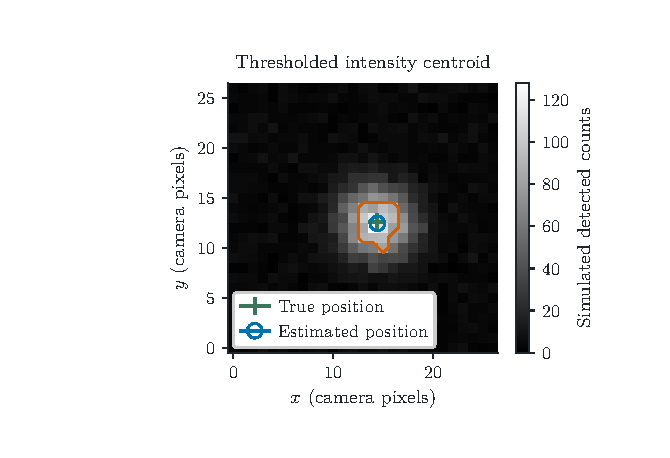
\includegraphics[width=0.70\linewidth]{T7_centroid}
  \caption{A synthetic pixel-integrated Gaussian spot with Poisson noise. The orange contour marks the $q=0.98$ threshold mask; the plus and circle distinguish truth and the application centroid. Subpixel coordinates do not imply zero error. This example uses no background correction.}
  \label{fig:centroid}
\end{figure}

\subsection{Localization precision (background)}
\label{sec:precision}

Because of photon noise (\cref{sec:noise}), repeating the measurement gives a
slightly different $\hat{x}_0$ each time. The spread of those estimates is the
\emph{localization precision}, written here as the standard deviation of a single position estimate,
$\mathrm{SE}$ (not the standard error of the mean of repeated estimates). A widely used closed-form estimate is the Thompson-Larson-Webb
formula~\cite{thompson2002}:
\begin{equation}
  \mathrm{SE} \approx \sqrt{\;\frac{\sigma^{2} + a^{2}/12}{N}
                        \;+\; \frac{8\pi\,\sigma^{4}\,b_{\mathrm{rms}}^{2}}{a^{2}\,N^{2}}\;},
  \label{eq:thompson}
\end{equation}
where $\sigma$ is the PSF width, $a$ the pixel size, $N$ the number of signal
photons, and $b_{\mathrm{rms}}$ the RMS background noise per pixel in
photon-equivalent units, distinct from the mean background $b$ in the forward
model. Both $\sigma$ and $a$ use the same length unit. Camera gray levels
are not photon counts without a gain and noise calibration. This approximation
is a theoretical reference, not an uncertainty estimate reported by the thresholded centroid.
The formula has two terms:
\begin{itemize}
  \item the \textbf{photon term} $(\sigma^2+a^2/12)/N$ dominates when the signal
        is strong; precision improves as $1/\sqrt{N}$;
  \item the \textbf{background term} $8\pi\sigma^4 b_{\mathrm{rms}}^2/(a^2N^2)$ dominates when
        the signal is weak relative to the background.
\end{itemize}
\Cref{fig:precision} plots this behaviour.

\begin{csnote}[Worked example: resolution is not precision]
Take $\sigma = 1.5$~px and a bright spot, $N = 10^4$ photons, with negligible
background. The photon term gives $\mathrm{SE} \approx
\sqrt{(1.5^2)/10^4} \approx 0.015$~px, about one part in a hundred of the
blur width. With only $N = 100$ photons, $\mathrm{SE} \approx 0.15$~px. The
emitter is blurred over several pixels, yet its \emph{centre} is known to a tiny
fraction of a pixel. This distinction underlies localization microscopy:
\emph{resolution} (the blur width, \cref{eq:abbe}) and \emph{precision} (how
well one centre is known, \cref{eq:thompson}) are different quantities, and the
second can be far smaller than the first.
\end{csnote}

\begin{figure}[htbp]
  \centering
  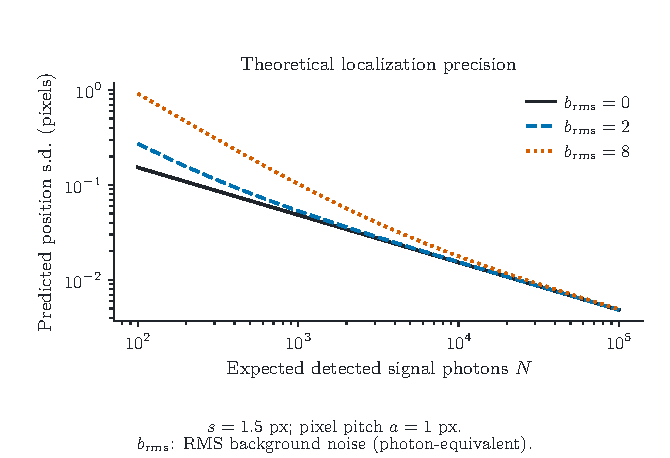
\includegraphics[width=0.70\linewidth]{T6_precision_vs_photons}
  \caption{The Thompson-Larson-Webb approximation is a theoretical reference, not an uncertainty estimate reported by the centroid software. The PSF width is $\sigma=1.5$ camera pixels, and the pixel pitch is $a=1$ in the same length units. $b_{\mathrm{rms}}$ is the RMS background noise, not the mean background. The standard deviation of position estimates scales as $N^{-1/2}$ in the signal-limited regime and $N^{-1}$ in the background-limited regime.}
  \label{fig:precision}
\end{figure}

\subsection{The statistical ideal (background only): MLE and the Cram\'er-Rao bound}
\label{sec:ideal}

\begin{csideal}
The centroid of \cref{eq:centroid} is transparent but can be biased by
thresholding, background, or overlapping spots. A model-based alternative is
maximum-likelihood estimation. For independent Poisson pixels, it minimizes
\begin{equation}
  L(\theta)=\sum_{i,j}[M_{ij}(\theta)-Z_{ij}\ln M_{ij}(\theta)],
  \label{eq:nll}
\end{equation}
up to terms independent of $\theta=(x_0,y_0,N,b,\sigma)$. Under the usual
regularity conditions, an unbiased estimator obeys the Cram\'er-Rao covariance
bound~\cite{ober2004,mortensen2010}:
\begin{equation}
  \operatorname{Cov}(\hat\theta)\succeq F^{-1},\qquad
  F_{mn}=\sum_{i,j}\frac{1}{M_{ij}}
  \frac{\partial M_{ij}}{\partial\theta_m}
  \frac{\partial M_{ij}}{\partial\theta_n}.
  \label{eq:crlb}
\end{equation}
The matrix inequality means that the covariance difference is positive
semidefinite. Maximum-likelihood estimators can approach the bound in an
appropriate large-sample regime with the correct model; finite-sample
attainment is not guaranteed. A biased thresholded centroid is not generally
covered by this simple unbiased bound. V1.2 implements neither this optimizer
nor per-event Fisher-information uncertainty. These equations describe a
possible extension, not a fitted stage in the present pipeline.
\end{csideal}

% ======================================================================
\section{Precision versus Accuracy}
\label{sec:precacc}

Two estimates can be tightly clustered yet systematically wrong. It is essential
to keep two ideas separate~\cite{deschout2014}:
\begin{description}[leftmargin=1.6em]
  \item[Precision] is \emph{repeatability}, or how closely repeated measurements
        of the same emitter agree with one another. It is the random scatter,
        and it is what \cref{eq:thompson} estimates.
  \item[Accuracy] is \emph{correctness}, or how close the estimates are to the
        \emph{true} position. A constant offset (a bias) reduces accuracy without reducing precision.
\end{description}
\Cref{fig:precacc} contrasts the two. The background bias of the V1.2 centroid
(\cref{sec:centroid}) is an accuracy problem: it can shift estimates
without widening their scatter. This is why \app{}'s \emph{Virtual Experiment}
saves the true positions in \file{truth.csv}: comparing reconstructed positions
against the truth measures \emph{accuracy}, which precision alone cannot reveal.

\begin{figure}[htbp]
  \centering
  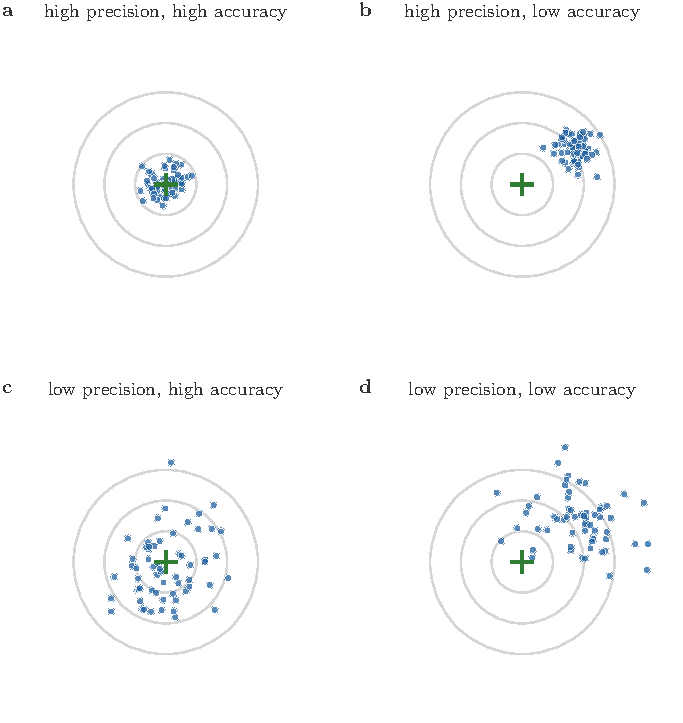
\includegraphics[width=0.72\linewidth]{T8_precision_accuracy}
  \caption{Illustrative samples separate repeatability (spread) from systematic offset (bias). The mean is explicitly controlled. Accuracy depends on both bias and random error; small spread alone is not accuracy.}
  \label{fig:precacc}
\end{figure}

% ======================================================================
\section{From Localizations to a Reconstructed Image}
\label{sec:rendering}

A list of localized positions is not yet a picture. \app{} \emph{renders} it:
each accepted localization is drawn as a small Gaussian ``splat,'' and all the
splats are summed into the super-resolution image. In V1.2 every splat is drawn
with the same fixed width (about $1.5$~px); the splat width is a display choice
that makes the sparse points visible, not a measurement.
The Gaussian is evaluated at the fractional localization coordinate without
rounding its centre to an integer pixel. Each displayed kernel is normalized
to unit sum, including at a boundary. The output grid retains the camera pixel
spacing; neither the display width nor its sampling establishes resolution.

Spatial coverage is independent of position precision. For an ideal,
regularly sampled, band-limited signal with smallest spatial period $d$, the
Nyquist condition is
\begin{equation}
  \Delta_s \le d/2,
  \label{eq:nyquist}
\end{equation}
where $\Delta_s$ is the sampling pitch, not the localization uncertainty.
Irregular SMLM labeling requires additional care: repeated blinking can revisit
the same site without filling gaps, and an average nearest-neighbor distance
alone does not guarantee adequate coverage~\cite{prakash2024,lelek2021}.
\Cref{fig:nyquist} illustrates coverage at fixed positional noise; it does not
establish a universal resolution criterion.

\begin{figure}[htbp]
  \centering
  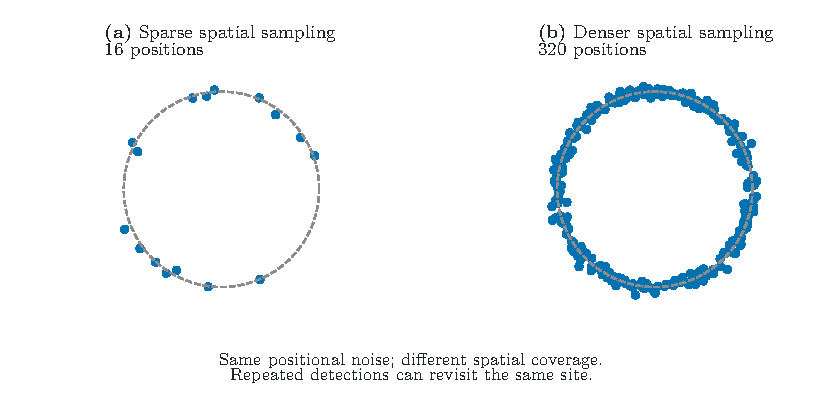
\includegraphics[width=0.86\linewidth]{T9_nyquist}
  \caption{Synthetic ring sampled at 16 or 320 independently drawn positions with the same radial noise. Sampling spacing and localization precision are different quantities. No universal resolution threshold or adequate sample count is inferred from this illustration.}
  \label{fig:nyquist}
\end{figure}

\begin{cswarn}[Reporting resolution]
The width of a rendered splat is \emph{not} the resolution of the result. Good reporting practice~\cite{prakash2024} is to report the localization precision
(\cref{eq:thompson}) and the sampling density (\cref{eq:nyquist}) separately,
rather than quoting a single number. \app{} is designed to make both visible
rather than to report a single summary value.
\end{cswarn}

% ======================================================================
\section{The \app{} V1.2 Pipeline}
\label{sec:pipeline}

The list below describes what \app{} V1.2 does
when you click \emph{Run Reconstruction} (\cref{fig:pipeline}). The steps connect the procedure to the equations above.

\begin{enumerate}
  \item \textbf{Load} the blinking video frame by frame (optionally cropped).
  \item \textbf{Preprocess} with optional frame-median background subtraction;
        keep the uncorrected frames for the raw mean. Constant frames yield
        no localizations.
  \item \textbf{Threshold} each frame: pixels brighter than a high intensity
        percentile (the top $0.5\%$ by default) form the candidate mask $\mathcal{M}$.
  \item \textbf{Localize} with the intensity-weighted centroid of
        \cref{eq:centroid}, once per frame in \texttt{single} mode, or once
        per separated bright region in \texttt{multiple} mode.
  \item \textbf{Accumulate} the localizations from all frames.
        Retain crop-local and original-frame coordinates. If calibration is
        supplied, multiply original-frame coordinates by the physical scale
        and export the calibrated columns and unit label.
  \item \textbf{Render} each localization as a Gaussian splat
        ($\sigma \approx 1.5$~px) and sum them into the super-resolution image.
  \item \textbf{Average} the frames separately to form the diffraction-limited
        \emph{raw mean} image.
  \item \textbf{Compare} the raw mean and the reconstruction, using, for example, the linked profile viewer.
\end{enumerate}

The \emph{linked profile viewer} lets you compare the two images using profiles through a chosen point. Writing $I(x,y)$ for an image and $(x_0,y_0)$ for the chosen point,
the viewer plots the row and column profiles
\begin{equation}
  I_x(x) = I(x,y_0), \qquad I_y(y) = I(x_0,y),
  \label{eq:profile}
\end{equation}
for both the raw mean and the reconstruction. These profiles compare the
displayed images. Their widths and valley depths depend on the rendering
kernel and normalization, so narrow reconstructed peaks alone do not establish
resolution. \Cref{fig:rawvssr} instead uses known source positions and a
reproducible synthetic run; position errors are assessed against that truth.

\begin{figure}[htbp]
  \centering
  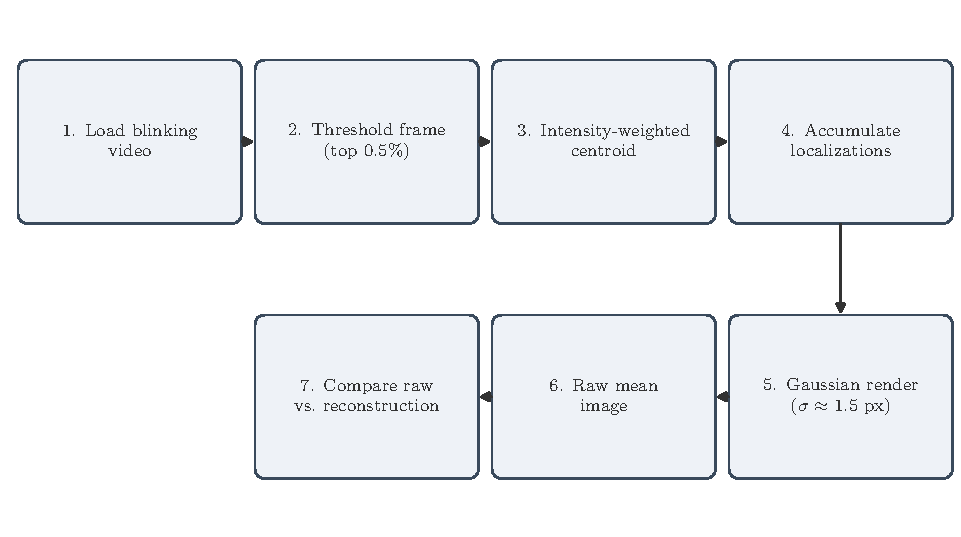
\includegraphics[width=\linewidth]{T10_pipeline}
  \caption{The current centroid pipeline, with a separate raw-mean branch. The rendering width is fixed and is not an uncertainty estimate.}
  \label{fig:pipeline}
\end{figure}

\begin{figure}[htbp]
  \centering
  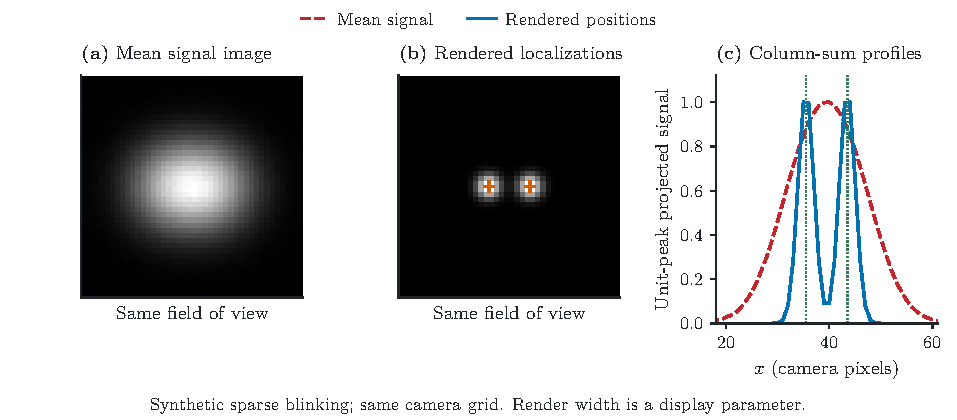
\includegraphics[width=\linewidth]{T11_raw_vs_reconstruction}
  \caption{Actual V1.2 centroid reconstruction of 600 synthetic pixel-integrated Poisson frames. Exactly one of two sources is active per frame. The separation is 8 pixels, and the optical Gaussian width is $\sigma=6$ pixels. The threshold is $q=0.995$, with frame-median subtraction. The known simulated background is subtracted from the mean image for display. Both images and column-sum profiles are independently peak-normalized. Green guides and orange crosses mark the true positions. The Gaussian rendering width of $\sigma_r=1.5$ pixels does not measure resolution. Source data and run parameters accompany the figure.}
  \label{fig:rawvssr}
\end{figure}

% ======================================================================
\section{Scope, Assumptions, and Limitations}
\label{sec:limitations}

\app{} V1.2 is a teaching tool. Each limitation below provides a topic for student discussion.

\begin{cswarn}[What \app{} V1.2 does and does not do]
\begin{itemize}
  \item \textbf{Overlapping emitters cannot be separated.} If two spots merge,
        the centroid of the merged region returns a single incorrect position
        (\cref{sec:blinking}). Reliable reconstruction needs sparse, separated
        blinking.
  \item \textbf{The centroid gives a position but no uncertainty.} V1.2 does not
        compute a per-localization standard error. \Cref{eq:thompson} tells you
        what precision to \emph{expect}; the software does not report it spot by
        spot.
  \item \textbf{Limited background correction.} Optional frame-median
        subtraction assumes sparse emitters and does not model gradients or
        camera-specific noise.
  \item \textbf{No model fitting.} V1.2 does not perform weighted-least-squares
        or maximum-likelihood Gaussian fitting; it does not evaluate the
        Cram\'er-Rao bound.
  \item \textbf{The render width is fixed.} Every splat is drawn at the same
        width; it shows where localizations are, not the precision of each localization.
  \item \textbf{No drift correction.} Optional physical calibration rescales
        exported coordinates but does not correct motion or estimate precision.
  \item \textbf{Noisy, saturated, or underexposed video reconstructs poorly},
        because thresholding (\cref{sec:noise}) can no longer separate signal
        from noise.
\end{itemize}
These are deliberate simplifications that make every step easy to follow. They are
the starting points for the extensions below.
\end{cswarn}

% ======================================================================
\section{Extensions and Further Reading}
\label{sec:extensions}

The V1.2 method can be improved in well-understood ways; these are standard in
research SMLM and can serve as project extensions. They are \emph{not} part of
\app{} Studio V1.2.

\begin{itemize}
  \item \textbf{Local background estimation}, for example an annular median,
        can extend the current frame-median option when its assumptions fail.
  \item \textbf{Gaussian fitting.} Replacing the centroid with a weighted
        least-squares or maximum-likelihood fit of the model in
        \cref{eq:pixmodel} approaches the Cram\'er-Rao bound
        (\cref{eq:crlb}) and yields a per-localization
        precision~\cite{mortensen2010, small2014}.
  \item \textbf{Drift correction.} Slow stage drift can be measured by
        cross-correlating frames and subtracted before
        rendering~\cite{guizar2008}.
  \item \textbf{Resolution metrics.} Fourier ring correlation gives an
        image-based resolution estimate from two independent halves of the
        data~\cite{prakash2024}.
  \item \textbf{Reference software.} Research packages such as
        ThunderSTORM~\cite{ovesny2014} implement the full pipeline and are
        useful for comparison. An accessible introduction to SMLM data analysis
        is given by Lee \emph{et al.}~\cite{lee2017}, and the mathematical
        theory of recovering point sources is treated by Cand\`es and
        Fern\'andez-Granda~\cite{candes2014}.
\end{itemize}

% ======================================================================
\appendix

\section{A Short Derivation: Why Precision Scales as
         \texorpdfstring{$1/\sqrt{N}$}{1/sqrt(N)}}
\label{sec:appderiv}

\begin{csderiv}
A localization is, in essence, an average of the positions where the $N$
signal photons arrived. Each photon lands at a random position drawn from the
PSF, which has a spread of order $\sigma$. The standard error of the mean of $N$
independent samples, each with spread $\sigma$, is
\begin{equation*}
  \mathrm{SE} \approx \frac{\sigma}{\sqrt{N}}.
\end{equation*}
This is the leading (photon-limited) term of the Thompson formula,
\cref{eq:thompson}; the $a^2/12$ correction accounts for the finite pixel size,
and the second term accounts for background photons that carry no position
information. The lesson is simple and general: \emph{collect more photons and
the position estimate becomes more precise, in proportion to the square root of the count.}
\end{csderiv}

\section{Symbol Table}
\label{sec:symbols}

\begin{table}[htbp]
\centering\small
\begin{tabularx}{\linewidth}{@{}lX@{}}
\toprule
\textbf{Symbol} & \textbf{Meaning}\\
\midrule
$\lambda$ & Wavelength of light\\
$\mathrm{NA}$ & Numerical aperture of the imaging lens\\
$d_{\mathrm{Abbe}},\,d_{\mathrm{Rayleigh}}$ & Diffraction-limited resolution
  (\cref{eq:abbe,eq:rayleigh})\\
$h,\,f,\,g$ & Point spread function, true scene, recorded image
  (\cref{eq:convolution})\\
$\sigma$ & Width of the (Gaussian) point spread function\\
$(x_0,y_0)$ & True position of an emitter; $(\hat{x}_0,\hat{y}_0)$ is its estimate\\
$N$ & Number of signal photons from an emitter\\
$b$ & Background level per pixel\\
$a$ & Camera pixel size\\
$M_{ij}$ & Expected counts in pixel $(i,j)$ (\cref{eq:pixmodel})\\
$Z_{ij}$ & Recorded counts in pixel $(i,j)$\\
$\sigma_{\mathrm{read}},\,g$ & Camera read noise and gain\\
$\mathcal{M}$ & Set of thresholded (candidate spot) pixels\\
$\mathrm{SE}$ & Single-position standard deviation\\
$L(\theta),\,F$ & Negative log-likelihood and Fisher information
  (\cref{eq:nll,eq:crlb})\\
\bottomrule
\end{tabularx}
\caption{Symbols used in these notes.}
\label{tab:symbols}
\end{table}

% ======================================================================
\begin{thebibliography}{99}
\addcontentsline{toc}{section}{References}

\bibitem{abbe1873} E.~Abbe, ``Beitr\"age zur Theorie des Mikroskops und der
  mikroskopischen Wahrnehmung,'' \textit{Archiv f\"ur Mikroskopische Anatomie}
  \textbf{9}, 413-468 (1873).

\bibitem{rust2006} M.~J.~Rust, M.~Bates, and X.~Zhuang, ``Sub-diffraction-limit
  imaging by stochastic optical reconstruction microscopy (STORM),''
  \textit{Nature Methods} \textbf{3}, 793-795 (2006).

\bibitem{betzig2006} E.~Betzig \textit{et al.}, ``Imaging intracellular
  fluorescent proteins at nanometer resolution,'' \textit{Science} \textbf{313},
  1642-1645 (2006).

\bibitem{hell1994} S.~W.~Hell and J.~Wichmann, ``Breaking the diffraction
  resolution limit by stimulated emission: stimulated-emission-depletion
  fluorescence microscopy,'' \textit{Optics Letters} \textbf{19}, 780-782
  (1994).

\bibitem{hell2007} S.~W.~Hell, ``Far-field optical nanoscopy,''
  \textit{Science} \textbf{316}, 1153-1158 (2007).

\bibitem{thompson2002} R.~E.~Thompson, D.~R.~Larson, and W.~W.~Webb, ``Precise
  nanometer localization analysis for individual fluorescent probes,''
  \textit{Biophysical Journal} \textbf{82}, 2775-2783 (2002).

\bibitem{mortensen2010} K.~I.~Mortensen, L.~S.~Churchman, J.~A.~Spudich, and
  H.~Flyvbjerg, ``Optimized localization analysis for single-molecule tracking
  and super-resolution microscopy,'' \textit{Nature Methods} \textbf{7},
  377-381 (2010).

\bibitem{ober2004} R.~J.~Ober, S.~Ram, and E.~S.~Ward, ``Localization accuracy
  in single-molecule microscopy,'' \textit{Biophysical Journal} \textbf{86},
  1185-1200 (2004).

\bibitem{deschout2014} H.~Deschout \textit{et al.}, ``Precisely and accurately
  localizing single emitters in fluorescence microscopy,'' \textit{Nature
  Methods} \textbf{11}, 253-266 (2014).

\bibitem{small2014} A.~Small and S.~Stahlheber, ``Fluorophore localization
  algorithms for super-resolution microscopy,'' \textit{Nature Methods}
  \textbf{11}, 267-279 (2014).

\bibitem{ovesny2014} M.~Ovesn\'y, P.~K\v{r}\'i\v{z}ek, J.~Borkovec,
  Z.~\v{S}vindrych, and G.~M.~Hagen, ``ThunderSTORM: a comprehensive ImageJ
  plug-in for PALM and STORM data analysis and super-resolution imaging,''
  \textit{Bioinformatics} \textbf{30}, 2389-2390 (2014).

\bibitem{guizar2008} M.~Guizar-Sicairos, S.~T.~Thurman, and J.~R.~Fienup,
  ``Efficient subpixel image registration algorithms,'' \textit{Optics Letters}
  \textbf{33}, 156-158 (2008).

\bibitem{schermelleh2019} L.~Schermelleh \textit{et al.}, ``Super-resolution
  microscopy demystified,'' \textit{Nature Cell Biology} \textbf{21}, 72-84
  (2019).

\bibitem{lelek2021} M.~Lelek \textit{et al.}, ``Single-molecule localization
  microscopy,'' \textit{Nature Reviews Methods Primers} \textbf{1}, 39 (2021).

\bibitem{sigal2018} Y.~M.~Sigal, R.~Zhou, and X.~Zhuang, ``Visualizing and
  discovering cellular structures with super-resolution microscopy,''
  \textit{Science} \textbf{361}, 880-887 (2018).

\bibitem{huang2010} B.~Huang, H.~Babcock, and X.~Zhuang, ``Breaking the
  diffraction barrier: super-resolution imaging of cells,'' \textit{Cell}
  \textbf{143}, 1047-1058 (2010).

\bibitem{lee2017} S.~Lee, T.~Tsekouras, C.~Calderon, C.~Bustamante, and
  S.~Press\'e, ``Unraveling the thousand word picture: an introduction to
  super-resolution data analysis,'' \textit{Chemical Reviews} \textbf{117},
  7276-7330 (2017).

\bibitem{prakash2024} K.~Prakash \textit{et al.}, ``Resolution in
  super-resolution microscopy: definition, trade-offs and perspectives,''
  \textit{Nature Methods} (2024), DOI:\,10.1038/s41592-024-02287-y.

\bibitem{danial2022} J.~S.~H.~Danial \textit{et al.}, ``Constructing a
  cost-efficient, high-throughput and high-quality single-molecule localization
  microscope for super-resolution imaging,'' \textit{Nature Protocols}
  \textbf{17}, 2570-2619 (2022).

\bibitem{ma2017} H.~Ma \textit{et al.}, ``A simple and cost-effective setup for
  super-resolution localization microscopy,'' \textit{Scientific Reports}
  \textbf{7}, 1542 (2017).

\bibitem{bechhoefer2015} J.~Bechhoefer, ``What is superresolution
  microscopy?,'' \textit{American Journal of Physics} \textbf{83}, 22-29
  (2015).

\bibitem{candes2014} E.~J.~Cand\`es and C.~Fern\'andez-Granda, ``Towards a
  mathematical theory of super-resolution,'' \textit{Communications on Pure and
  Applied Mathematics} \textbf{67}, 906-956 (2014).

\end{thebibliography}

\end{document}
